\documentclass{article}
%\usepackage[top=2.5cm, bottom=2.5cm, left=2.5cm, right=2.5cm]{geometry}
\usepackage[utf8]{inputenc}
\usepackage{amstext}
%\usepackage{times}
%\usepackage{ngerman}
\usepackage{amsmath}
\usepackage{amstext}
\usepackage{amssymb}
\usepackage{amsfonts}
\usepackage{bbm}
\usepackage{amsthm}
\usepackage{graphicx}
\usepackage{multirow}
\usepackage{booktabs}
\usepackage{enumerate}
\usepackage{multirow}
\usepackage{varwidth}
\usepackage{booktabs} 
\usepackage{rotating}
\usepackage{caption}
\usepackage{ifthen}
\usepackage{url}
\usepackage[ruled,lined]{algorithm2e}

\newenvironment{li}{\begin{itemize}\setlength{\itemsep}{-0.7ex}}{\end{itemize}}

\newcommand{\ie}{i.e.\ }
\newcommand{\eg}{e.g.\ }
\newcommand{\wrt}{w.r.t.\ }

\newcommand{\nxt}{\smallskip \noindent $\circ$ }

\DeclareMathOperator*{\argmax}{arg\,max}

\theoremstyle{definition}
\newtheorem{definition}{Definition}
\newtheorem{lemma}{Lemma}
\newtheorem{claim}{Claim}
\newtheorem{theorem}{Theorem}
\newtheorem{example}{Example}

\parskip=1ex

\begin{document}

\date{}
\author{Tobias Hochwallner, Lukas Lang}
\title{The Minimum Energy Broadcast Problem}
\maketitle

\section{Introduction}

Given a set of nodes $V$, a set of coordinates $C$ in the $2$-dimensional metric space and a surjective function $h: V \rightarrow C$, the \emph{Minimum Energy Broadcast Problem (MEBP)} is to find a spanning tree $T = (V, E_{T})$ with a fixed root $s \in V$ such that
\begin{equation}
	\sum_{i \in V} \max_{(i,j) \in E_{T}} d_{ij}^{l}
\end{equation}
is minimal. In the course of this work, we developed an \emph{Ant Colony Optimization (ACO)} algorithm for the MEBP. Furthermore, we subsequently applied local search.

\section{Ant Colony Optimization}

We implemented a basic version of ACO which is as follows: Each ant $1 \leq k \leq m$ keeps in each iteration a set of visited nodes $U_{k} \subseteq V$ and a neighborhood $\mathcal{N}_{k} := V \setminus U_{k}$ of unvisited nodes. Initially, $U_{k} = \{s\}$. Then in each iteration, the ant starts from a visited node $i \in U_{k}$, chosen uniformly at random, and runs to a random node $j \in \mathcal{N}_{k}$ according to the probability distribution $D_{i}$ reflected to the pheromone trails running from $i$ to $\mathcal{N}_{k}$. Moreover, we used the strategy \emph{Min-Max} to update the pheromone trails. The pseudocode of the algorithm can be found in Algorithm \ref{alg:aco}.

\begin{algorithm}
	\KwData{Graph $G = (V, E)$, number of ants $m$, number of iterations $t_{max}$.}
	\For{$t \gets 1,\dots,t_{max}$} {
		\ForEach{ant $k = 1,\dots,m$} {
			\While{$|\mathcal{N}^{k}| > 0$} {
				Select start node $i \in U_{k}$ uniform at random\;
				Select end node $j \in \mathcal{N}^{k}$ according to $p_{ij}$\;
				Add $(i,j)$ to solution\;
				$U_{k} \gets U_{k} \cup j$\;
			}
		}
		Update pheromones according to solution $\max_{k} f_{t}^{k}$\;
		Vaporize pheromones\;
	}
\caption{ACO pseudocode.}
\label{alg:aco}
\end{algorithm}

\section{Improvement Heuristic}

We decided to implement the \emph{Expanding Sweep Search} improvement heuristic as described in \cite{Kang2005}. The heuristic tries for each node $u \in V$ to increase the transmission power to every node $v \in V$ and $u \neq v$ such that nodes in other cells are covered by $i$. Figure \ref{fig:sweep} shows a single expansion step.

\begin{figure}[h]
	\begin{center}
	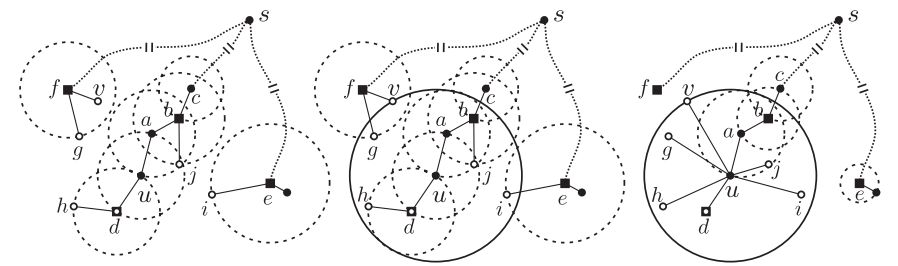
\includegraphics[width=12cm]{images/sweepsearch.png}
	\end{center}
	\caption{Expanding Sweep Search.} \label{fig:sweep}
\end{figure}

\section{Experimental Results}

We created an automated evaluation framework and performed several test runs for the implementation. Since in some cases the improvement heuristic could not manage to repair damaged solutions, we only took valid solutions. The parameters of the framework were set as follows:

\begin{center}
\begin{tabular}{|l|r|}
	\hline
	\textbf{Parameter} & \textbf{Value} \\
	\hline
	Runs & 10 \\
	\hline
	Iterations & 500 \\
	\hline
	Number of ants & 100 \\
	\hline
	$\rho$ & 0.5 \\
	\hline
	$\alpha$ & 0.5 \\
	\hline
	$\beta$ & 0.5 \\
	\hline
	$\tau_{init}$ & 2 \\
	\hline
	$\tau_{max}$ & 2 \\
	\hline
	$\tau_{min}$ & 0.5 \\
	\hline
\end{tabular}
\end{center}
The subsequent tables show the obtained results for the three tested instances with and without the expanding sweep heuristic, respectively.
\begin{center}
\begin{tabular}{|l|c|c|c|c|c|}
	\hline
	\textbf{Instance} & \footnotesize $n$ & \footnotesize $f_{min}$ & \footnotesize $f_{max}$ & \footnotesize $\bar f$ & \footnotesize $\sigma^{2}$ \\
	\hline
	mebp-06 & 4 & $2.3466\cdot10^{8}$ & $2.7490\cdot10^{8}$ & $2.6019\cdot10^{8}$ & $3.1552\cdot10^{14}$ \\
	\hline
	mebp-08 & 9 & $2.9373\cdot10^{8}$ & $4.2871\cdot10^{8}$ & $3.6746\cdot10^{8}$ & $1.5217\cdot10^{15}$ \\
	\hline
	mebp-10* & & & & \\
	\hline
	\multicolumn{6}{|l|}{* result was obtained using 100 iterations and 50 ants.} \\
	\hline
\end{tabular}
\end{center}
The following results were obtained \textbf{without} the improvement heuristic:

\begin{center}
\begin{tabular}{|l|c|c|c|c|c|}
	\hline
	\textbf{Instance} & \footnotesize $n$ & \footnotesize $f_{min}$ & \footnotesize $f_{max}$ & \footnotesize $\bar f$ & \footnotesize $\sigma^{2}$ \\
	\hline
	mebp-06 & 10 & $2.2007\cdot10^{8}$ & $3.064\cdot10^{8}$ & $2.7964\cdot10^{8}$ & $7.3399\cdot10^{14}$ \\
	\hline
	mebp-08 & 10 & $3.7396\cdot10^{8}$ & $4.2124\cdot10^{8}$ & $3.9075\cdot10^{8}$ & $3.0453\cdot10^{14}$ \\
	\hline
	mebp-10 & 5 & $4.2275\cdot10^{8}$ & $4.5718\cdot10^{8}$ & $4.46\cdot10^{8}$ & $1.203\cdot10^{14}$ \\
	\hline
\end{tabular}
\end{center}

\section{Conclusion}

We created a framework to solve the Minimum Broadcast Energy Problem using Ant Colony Optimization. Furthermore, we implemented a simple improvement heuristic, namely the Expanding Sweep Search. Out of curiosity, we run experiments with $l=2$ and compared to the best known solutions\footnote{\url{http://dag.informatik.uni-kl.de/research/meb/}} which were found to be competitive.

\bibliographystyle{amsplain}
\bibliography{bibliography}

\end{document}